\section{Verification purpose}

\textbf{Case ID:} \CaseID

This case verifies Eulerian firebrand transport when wind varies in space and time. Surface spread, crosswind dispersion, consumption, and ignition delay are disabled so the leading edge follows a controlled characteristic equation.

The test exposes incorrect meteorology interpolation, direction conversion, tracker lifetime, or transport/level-set timestep coupling. Success requires leading-edge position and running-average spread rate to agree with an independently integrated characteristic solution.

\section{Mathematical formulation and numerical implementation}
The imposed one-dimensional velocity is
\begin{equation}
 u(x,t)=\bar u+A\sin\left(\frac{2\pi x}{\lambda_x}\right)
                 \sin\left(\frac{2\pi t}{T}\right),
 \quad
 (\bar u,A,\lambda_x,T)=(6.71,3.355,100,60)
\end{equation}
in SI units~\cite{Qin2025}. The exact leading edge is the characteristic satisfying
\begin{equation}
 \frac{dx_{\rm LE}}{dt}=u(x_{\rm LE},t),\qquad x_{\rm LE}(0)=5~{\rm m}.
\end{equation}
The postprocessor integrates this ODE with fourth-order Runge--Kutta and a
\SI{0.005}{s} substep.

The preprocessor samples the analytical wind every \SI{1}{s} into 121 bands of
\texttt{ws.tif}; \texttt{wd.tif} holds a constant 270-degree meteorological
direction. ELMFIRE linearly interpolates adjacent weather bands using
\texttt{DT\_METEOROLOGY}. The namelist explicitly selects \texttt{PER-AREA}
generation, \texttt{EULERIAN} accumulation, and \texttt{DIRECT} ignition.
Because surface fire is disabled, the per-area source avoids any dependence on
fireline intensity. Each ignited cell emits for \SI{10}{s}.

\section{Derivation of expected behavior}
The characteristic velocity is strictly positive:
$3.355\le u\le10.065~{\rm m\,s^{-1}}$, so the reference leading edge is
monotone. At each reporting time the simulated position is reconstructed as the
furthest centre-row cell whose final ELMFIRE arrival time is no later than that
time. Grid crossing makes the discrete instantaneous ROS alternate between zero
and approximately $\Delta x/\Delta t$. For the reference-aligned diagnostic, a centred
nine-point average should recover the smooth reference $u(x_{\rm LE}(t),t)$.

\section{Verification metrics and acceptance criteria}
For all finite samples, the postprocessor calculates mean and maximum absolute
position error, the mean absolute error of the nine-point running-average ROS,
and temporal coverage. The case passes only if
\[
 {\rm MAE}_x\le10~{\rm m},\quad
 \max|e_x|\le20~{\rm m},\quad
 {\rm MAE}_{\overline{\rm ROS}}\le2~{\rm m\,s^{-1}},\quad
 f_{\rm coverage}\ge0.90 .
\]
Missing or unusable output is explicitly non-passing.

\subsection{Justification of metric quantification}

The \SI{10}{m} position-MAE limit equals one grid cell, and the
\SI{20}{m} maximum limit equals two cells.  These bounds recognize that a
continuous characteristic is reconstructed from cell-centred arrival events
while still rejecting persistent phase errors.  Differentiation magnifies that
position quantization, so ROS is assessed after a centred nine-point average;
its \SI{2}{m.s^{-1}} allowance is smaller than the configured
\SI{3.355}{m.s^{-1}} velocity amplitude.  A run that merely reproduces the
mean wind but misses the oscillatory response therefore cannot satisfy the ROS
criterion.  The 90\% coverage requirement allows a small number of unmatched
samples near raster or temporal boundaries but prevents selective omission of
a substantial high-error portion of either wind cycle.  The four conditions
measure bias, worst local error, derivative fidelity, and sampling support,
respectively, so all are required for acceptance.

\subsection{Predeclared acceptance contract}

Table~\ref{tab:acceptance-contract} summarizes the metrics fixed before
inspection of the calculated results. Numerical values and component statuses
are reported separately in Section~7.

\begin{table}[H]
\centering
\footnotesize
\caption{Predeclared verification metrics and acceptance criteria.}
\label{tab:acceptance-contract}
\begin{tabular}{@{}p{0.23\linewidth}p{0.47\linewidth}p{0.21\linewidth}@{}}
\toprule
Metric & Output, region, and aggregation & Acceptance criterion\\
\midrule
Output completeness & Final TOA raster with valid physical centre-row coverage; two-cell halo and nodata are excluded. & Usable output required \\
Position MAE & Mean \(|x_{LE,ELMFIRE}(t)-x_{ODE}(t)|\) over finite matched samples. & \(\le\SI{10}{m}\) \\
Maximum position error & Maximum absolute leading-edge difference over the same samples. & \(\le\SI{20}{m}\) \\
Running-ROS MAE & Mean absolute error of the centred nine-point ELMFIRE ROS against the characteristic solution. & \(\le\SI{2}{m.s^{-1}}\) \\
Temporal coverage & Fraction of required characteristic times having finite ELMFIRE leading-edge observations. & \(\ge0.90\) \\
Overall decision & Conjunction of completeness and all four quantitative components. & PASS only if all pass \\
\bottomrule
\end{tabular}
\end{table}

\section{Simulation configuration and predicted outcome}

Figure~\ref{fig:input-configuration} records the prepared spatial inputs for the base time-dependent-wind run.
The postprocessor reads these panels from the variant-local GeoTIFF files, removes the
two-cell numerical buffer, and retains map coordinates in metres.  The left panel shows
the most informative fuel or structure layout available for the case; the right panel
shows the cells selected by the non-positive initial level-set field, making a localized
ignition or firebrand-emission source explicit.

\begin{figure}[H]
\centering

\includegraphics[width=0.98\textwidth,height=0.42\textheight,keepaspectratio]{../figures/input_configuration.pdf}
\caption{Whole-domain prepared input configuration for the representative variant.  The
physical domain is shown without the numerical halo; coordinates, configured wind values,
fuel or structure layout, and initial ignition/source geometry are identified in the panels.}
\label{fig:input-configuration}
\end{figure}

\begin{table}[htbp]
\centering
\caption{Configuration of the reconstructed time-dependent-wind case.}
\begin{tabular}{lll}
\toprule
Parameter & Value & Role\\
\midrule
Physical domain & \SI{1200}{m} by \SI{100}{m} & contains the 120-s trajectory\\
Cell size & \SI{10}{m} & streamwise discretization\\
Numerical halo & 2 cells per side & excluded from observations\\
Duration & \SI{120}{s} & two wind periods\\
Wind bands & 121 at \SI{1}{s} & time-varying forcing\\
Wind CFL & 0.5 & resolves wind transport\\
Generation & PER-AREA, \SI{1}{pcs\,m^{-2}\,s^{-1}} & no-surface source\\
Emission duration & \SI{10}{s} & fixed finite-duration source\\
Source selection & 100\% deterministic & removes sampling variability\\
Accumulation/ignition & EULERIAN/DIRECT & tested transport and ignition path\\
\bottomrule
\end{tabular}
\end{table}
The predicted position is a smooth monotone curve. Instantaneous numerical ROS
is grid-quantized, while its nine-point mean should follow the oscillatory ODE
velocity.

\section{Actual simulation results}

Figure~\ref{fig:domain-result} shows the representative time-of-arrival field from the base time-dependent-wind run.
It is read from the actual ELMFIRE output named in the panel, masks nodata, and excludes
the two-cell numerical buffer.  The field provides the spatial counterpart to the leading-edge history and reveals whether the changing wind produces a coherent transported front across the complete domain.

\begin{figure}[H]
\centering

\includegraphics[width=0.96\textwidth,height=0.50\textheight,keepaspectratio]{../figures/domain_result.pdf}
\caption{Whole-domain time-of-arrival field from the representative completed ELMFIRE run.  This
domain-scale result supplements, rather than replaces, the higher-level verification
profiles, convergence plots, ensemble statistics, and calculated acceptance metrics below.}
\label{fig:domain-result}
\end{figure}


Figure~\ref{fig:time-dependent-wind} first reproduces the two principal
time-dependent-wind observables. The numerical curves are reconstructed from
the final ELMFIRE arrival-time raster; the smooth curves are obtained by
integrating the prescribed leading-edge ODE.

\begin{figure}[H]
\centering
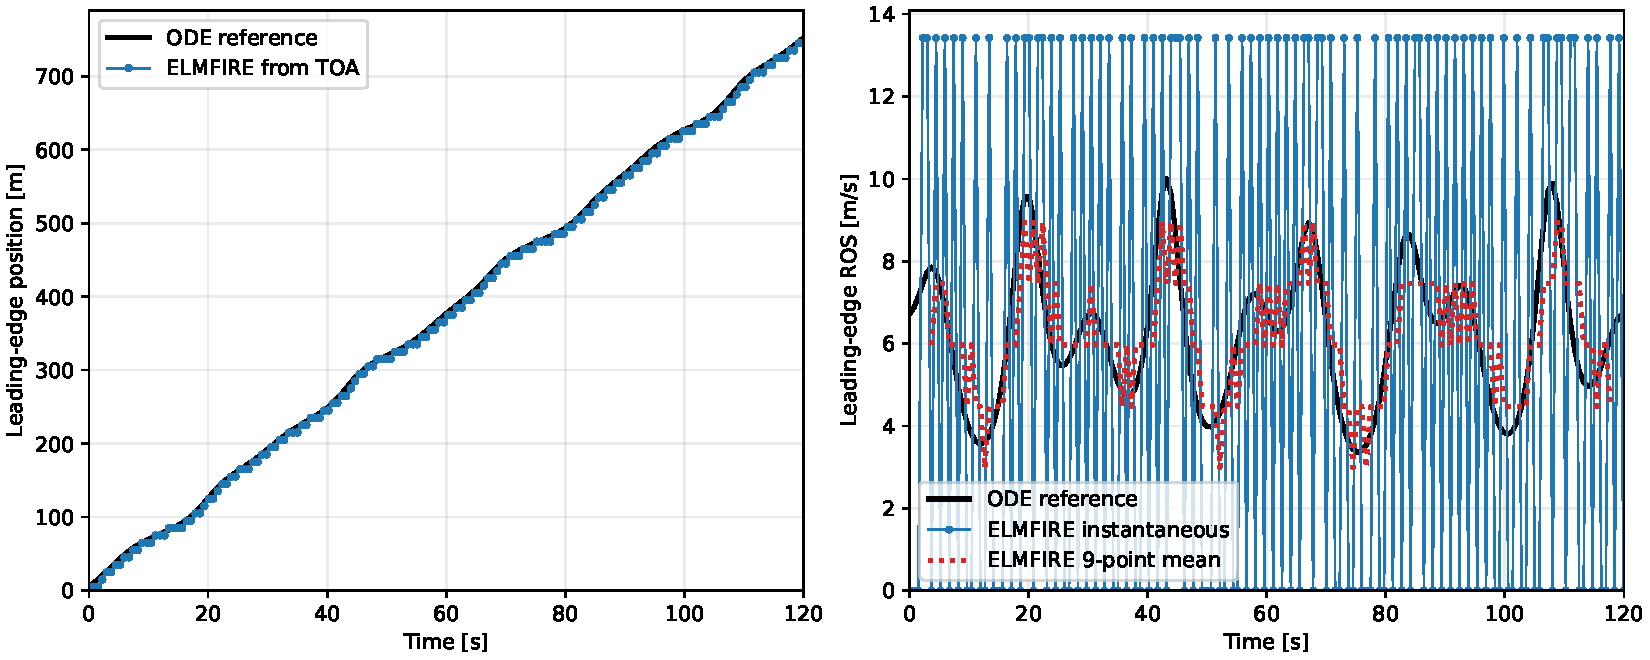
\includegraphics[width=\textwidth,height=0.42\textheight,keepaspectratio]
 {../figures/time_dependent_wind_transport.pdf}
\caption{Time-dependent-wind transport comparison. Left: ELMFIRE and ODE
leading-edge position. Right: ODE reference, grid-scale instantaneous ROS, and
the nine-point running-average ELMFIRE ROS.}
\label{fig:time-dependent-wind}
\end{figure}

Figure~\ref{fig:time-dependent-errors} adds the time-resolved residuals and
acceptance limits. It exposes localized phase errors that can be hidden by a
single mean value.

\begin{figure}[H]
\centering
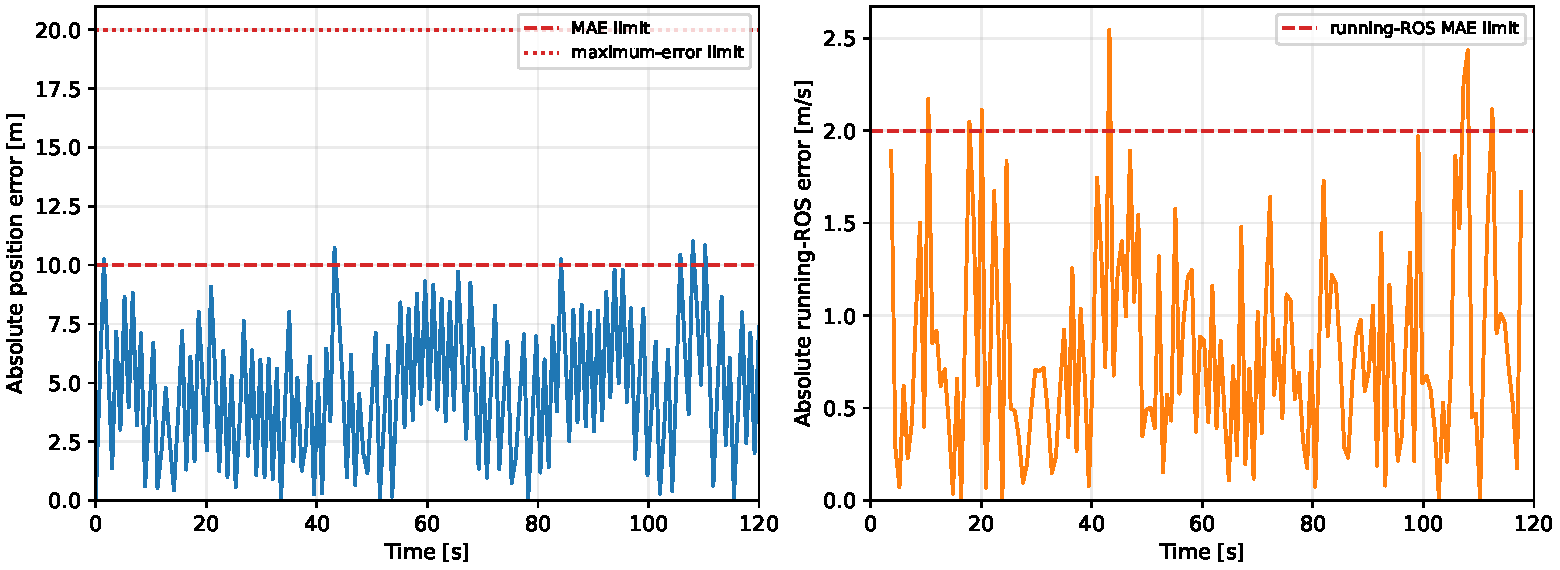
\includegraphics[width=0.94\textwidth,height=0.40\textheight,keepaspectratio]{../figures/time_dependent_wind_errors.pdf}
\caption{Absolute leading-edge-position and running-ROS errors through the
simulation. Horizontal lines identify the applicable acceptance limits.}
\label{fig:time-dependent-errors}
\end{figure}

\section{Calculated metrics and verification decision}
\begin{table}[htbp]
\centering
\caption{Acceptance metrics calculated by postprocessing.}
\begin{tabular}{llll}
\toprule
Metric & Limit & Calculated & Pass\\
\midrule
Position MAE & \(\le\)\SI{10}{m} & \Metric{positionmaem} & \Metric{positionmaepassed}\\
Position maximum error & \(\le\)\SI{20}{m} & \Metric{positionmaxerrorm} & \Metric{positionmaxerrorpassed}\\
Running ROS MAE & \(\le\)\SI{2}{m/s} & \Metric{runningrosmaemps} & \Metric{runningrosmaepassed}\\
Time coverage & \(\ge0.90\) & \Metric{timecoveragefraction} & \Metric{timecoveragepassed}\\
\bottomrule
\end{tabular}
\end{table}
The decision read directly from \texttt{outputs/metrics.json} is
\textbf{\Metric{status}} (\texttt{verification\_passed} =
\Metric{verificationpassed}).

\section{Technical interpretation}
The executed case is a genuine failed verification. The ELMFIRE leading edge reaches only \Metric{finalsimulatedpositionm} m at 120 s, whereas the ODE reference reaches \Metric{finalreferencepositionm} m. The position MAE is \Metric{positionmaem} m, so the discrepancy is much larger than the expected one-cell representation error. The TOA sequence advances plausibly at early time but develops long gaps after approximately 215 m. Input inspection confirms 121 wind bands spanning 3.355--10.065 m s and the deterministic source-selection percentage is explicit. The remaining evidence therefore points to the current handling of time-indexed wind along recursive Eulerian ember trackers or their source activation history, rather than to a constant-wind input or coordinate-comparison error. Instantaneous ROS remains intentionally grid-quantized; its nine-point mean is the smooth acceptance observable.

\section{Scope and limitations}
This is deterministic code verification of the Eulerian algorithm. It does not
validate the empirical landing-distance distribution, crosswind dispersion,
Lagrangian sampling, or physical ignition probability. One-second weather bands
approximate the continuous analytical forcing by ELMFIRE's native linear
interpolation.

\begin{thebibliography}{9}
\bibitem{Qin2025}
Y. Qin, \emph{A Physics-Based Eulerian Framework for Modeling Firebrand
Showering in Regional-Scale Wildland and Wildland--Urban Interface Fire
Simulations}, Ph.D. dissertation, University of Maryland, College Park, 2025.
\end{thebibliography}
